% !TEX encoding = UTF-8
% !TEX TS-program = pdflatex
% !TEX root = ../tesi.tex

%**************************************************************
\chapter{Introduzione}
\label{cap:introduzione}
%**************************************************************

Questa tesi descrive l'esperienza e il percorso lavorativo svolto presso l'azienda GRUPPO4 sotto la supervisione di Tobia Conforto.

%**************************************************************
\section{L'azienda}
Gruppo4 è una web agency Padovana, da oltre vent'anni ha accumulato competenze e l'esperienza necessaria per fornire soluzioni efficaci e innovative nel settore web. Mediante un modello organizzativo consolidato e certificato sviluppano applicazioni web che si distinguono per la chiarezza dell'interfaccia utente (UX/UI) e per la loro usabilità.

%**************************************************************
\section{Gli obiettivi del progetto}
L'obiettivo principale di questo progetto consiste nella realizzazione di un componente di interfaccia grafica per il web in Kotlin. Il componente deve essere una tabella pivot interattiva che permette ad un utente la possibilità di esplorare liberamente i \emph{big data} contenuti al suo interno. Oltre alla realizzazione del componente, questo progetto ha anche lo scopo di valutare l'efficacia di Kotlin nel realizzare interfacce utente per il web in quanto l'azienda utilizza Kotlin nello sviluppo di \gls{api}.

%**************************************************************
\section{Tabella pivot}
L'azienda mi ha fornito una descrizione accurata della tabella pivot, in particolare della sua struttura e delle sue funzionalità. Nelle prossime sottosezioni descriverò gli elementi che la compongono e le possibili interazioni con l'utente. Durante la discussione dei requisiti del componente, l'azienda mi ha fornito un accesso ad una istanza della loro applicazione correntemente in uso.
\begin{minipage}{\linewidth}
	\makebox[\linewidth] {
		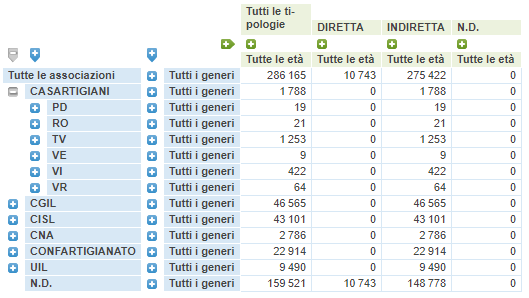
\includegraphics[scale=0.75]{./immagini/tabella-pivot-old.png}
	}
\end{minipage}

\subsection{Struttura}
La tabella pivot si può suddividere in tre parti ben distinte: le celle contenente i dati, le celle d'intestazione delle righe e quelle delle colonne. 
Le celle d'intestazione sono definite come le dimensioni della tabella. Ognuna di essa rappresenta tutti i campi dati riguardanti una tabella di un database che in seguito viene unita ad altre tabelle rappresentante dalle altre dimensioni in modo da ottenere l'intera tabella.

\subsection{Funzionalità}
La tabella deve essere completamente esplorabile da un utente. Come si può vedere dallo screenshot della tabella che sono presenti alcuni pulsanti. Essi servono per esguire due tipi di azioni: sulle dimensioni (tutti i figli di una dimensione possono essere aperti o chiusi contemporaneamente) e sulle singole celle di una dimensione (ogni cella di una dimensione deve poter essere aperta o chiusa con un semplice pulsante se essa presenta altri figli da renderizzare).

%**************************************************************
\section{Organizzazione del testo}
Riguardo la stesura di questo documento sono state adottate le seguenti convenzioni tipografiche:
\begin{itemize}
	\item gli acronimi, le abbreviazioni e i termini ambigui o di uso non comune menzionati vengono definiti nel glossario, situato alla fine del presente documento;
	\item per la prima occorrenza dei termini riportati nel glossario viene utilizzata la seguente nomenclatura: \emph{parola}\glo;
	\item i termini in lingua straniera o facenti parti del gergo tecnico sono evidenziati con il carattere \emph{corsivo}.
\end{itemize}